\documentclass[conference]{IEEEtran}
\usepackage{CJKutf8}
\usepackage{cite}
\usepackage{amsmath,amssymb,amsfonts}
\usepackage{algorithmic}
\usepackage{graphicx}
\usepackage{textcomp}
\usepackage{xcolor} 
\usepackage{multirow}
\def\BibTeX{{\rm B\kern-.05em{\sc i\kern-.025em b}\kern-.08em
    T\kern-.1667em\lower.7ex\hbox{E}\kern-.125emX}}
\begin{document} 
\begin{CJK}{UTF8}{bsmi}

\title{HW1 - GA in Numerical Optimization}
 
\author{
\IEEEauthorblockN{Sheng-Hsuan Peng}
\IEEEauthorblockA{
\textit{PME, NTHU} \\
107033588}}

\maketitle

\section{Objectives}
Practice and get familiar with the most widely used evolutionary algorithm — genetic algorithm
(GA). In this assignment you need to make use of the taught subject matters about GA’s
representation, crossover, mutation, and survivor to solve the given problem.

\section{Problem Description}
Write efficient programs to implement GAs to find the minimal solution of the Schwefel function
(SCH):

\begin{displaymath}
\mathop{f_{SCH}\left(\vec{x}\right)=418.98291N-{\sum_{i=1}^N}x_{i}\sin\left(\sqrt{|x_{i}|}\right)}
\end{displaymath}

where $-512\leq x_{i}\leq511$ and N = 10. This function is a continuous, multimodal, non-convex,
deceptive, and N-dimensional function with a global minimum of 0.

\begin{table}[htbp]
\caption{Parameters}
\begin{center}
\begin{tabular}{|c|c|c|}
\hline 
    & Binary GA & Real-valued GA\tabularnewline
\hline 
\hline 
Representation & $c_{i}$$\in$$2^{10}$ & $c_{i}$$\in$$\mathbb{R}$\tabularnewline
\hline 
Population & \multicolumn{2}{c|}{Generation (size 100)}\tabularnewline
\hline 
Parent Selection & \multicolumn{2}{c|}{Tournament Selection($\mathrel{n=2}$)}\tabularnewline
\hline 
\multirow{2}{*}{Crossover ($p_{c}=0.9$)} & \multicolumn{2}{c|}{Uniform}\tabularnewline
\cline{2-3} 
    & 2-point & Whole-Arithmetic\tabularnewline
\hline 
Mutation ($p_{m}=1/l$) & Bit-flip & Uniform\tabularnewline
\hline 
Survivor Selection & \multicolumn{2}{c|}{$\mu$$+\lambda$ }\tabularnewline
\hline 
Termination & \multicolumn{2}{c|}{500 generations}\tabularnewline
\hline 
\end{tabular}
\end{center}
\end{table}
    
\section{Result}

\begin{figure}[htbp]
%\centerline{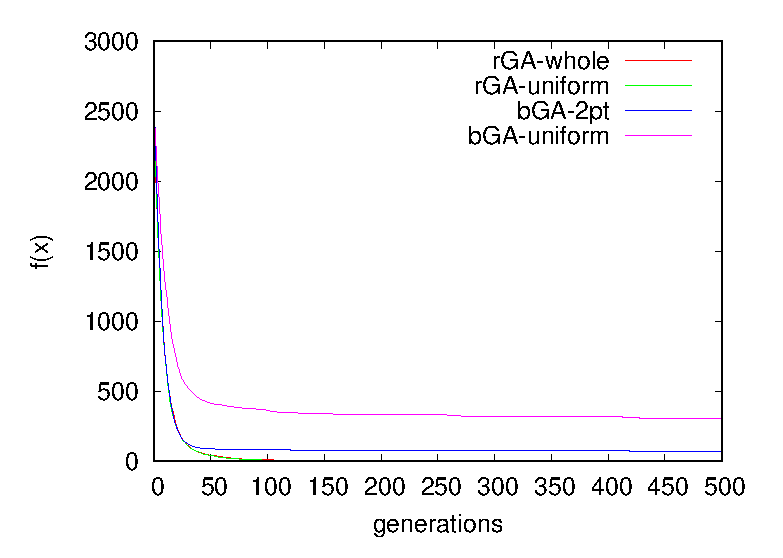
\includegraphics[width=\linewidth]{fig/cmp4GA/4GAs.eps}}
\centerline{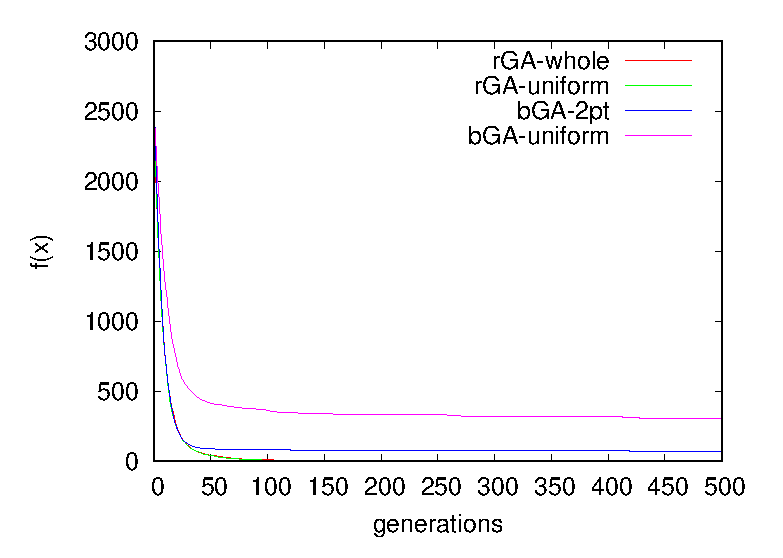
\includegraphics[width=7.5cm]{fig/cmp4GA/4GAs.eps}}
\caption{anytime behavior (averaged over 30 trials) of the above GAs}
\label{fig}
\end{figure}

\section{Comparison}
Compare convergence speed and solution quality between different representations and operators; give reasons why some combination performs better (or worse).

\subsection{Convergence Speed}
Real-valued GAs and Binary GA with 2-point crossover have same speed at the begin, and Binary GA with 2-point crossover converge first, then the 2 Real-valued GAs converge, then the Binary GA with uniform crossover.

\subsection{Solution Quality}
Real-valued GAs have better performance over the 4 GAs, and they could reach the optimum f(x) value (0). However, Binary GAs can't reach the optimum f(x) value, and Binary GA has the worst performance

\subsection{Reason}
The representation of the above GAs lead to these outcomes. For Binary GAs, changing of bits would have different degrees of influence due to it's location. Take 0000000000 as example, this gene has it's fitness -512, if the first bit changes to 1 (1000000000), then value would be 0, in the meanwhile, the change of last (0000000001) bit would only lead to the change of 1. And for Real-valued GAs the method of crossover would lead the children be the mid-fitness of their parents, thus would tend to evolute into the mid-point of the search space, which is 0 the optimum point. Thus Real-valued GAs would have better convergence speed and solution quality in this problem.

\section{Other Setting}
\subsection{Binary GA(Uniform Crossover)}
In this section, I had tried different parameters setting for $p_{c}, p_{m}, n$ 

\begin{figure}[htbp]
%\centerline{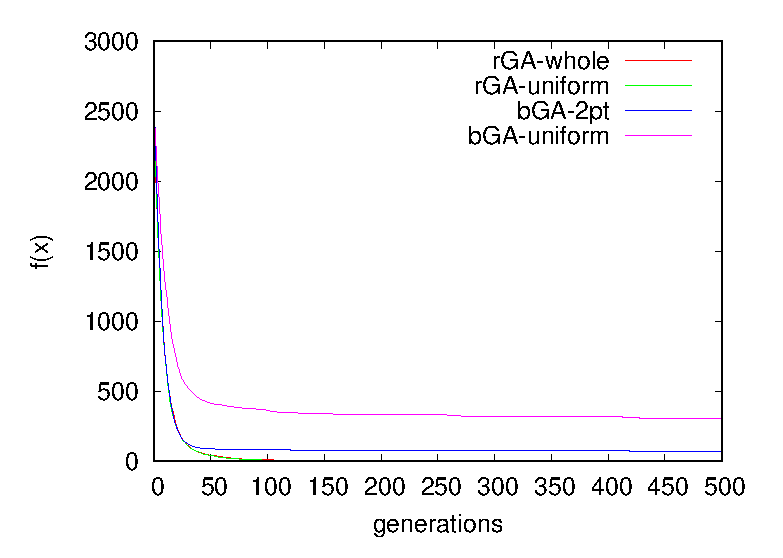
\includegraphics[width=\linewidth]{fig/cmp4GA/4GAs.eps}}
\centerline{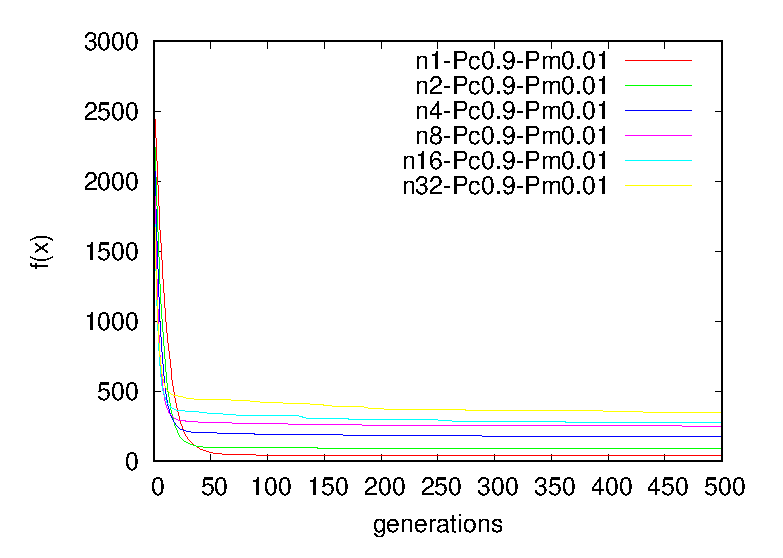
\includegraphics[width=7.5cm]{fig/bGA/change_n_2pt.eps}}
\caption{Binary GA(Uniform Crossover)}
\label{fig}
\end{figure}

\begin{itemize}
\item 需大量資料才可建立足夠信賴之model
\end{itemize}

\section{Expected Result}
建立一model能將加工參數與及時震動資料進行預測出預期加工品質。

\begin{thebibliography}{00}
\bibitem{b1} Jin, Yaochu, et al. ``Data-driven evolutionary optimization: An overview and case studies,'' IEEE Transactions on Evolutionary Computation, 2018.
\bibitem{b2} Wang, Handing, et al. ``Offline data-driven evolutionary optimization using selective surrogate ensembles.'' IEEE Transactions on Evolutionary Computation, 2018.
\bibitem{b3} Y.  Jin,  Ed., Knowledge  Incorporation  in  Evolutionary  Computation. Springer, 2005.

\end{thebibliography}
\vspace{12pt}
\end{CJK}
\end{document}
